\documentclass[preprint,12pt]{elsarticle}

\usepackage{amsmath,amssymb}
\usepackage{graphicx}
\usepackage{booktabs}
\usepackage{url}

\journal{European Journal of Mechanics - A/Solids}

\begin{document}

\begin{frontmatter}

\title{Granular penetration of a growing morphoelastic root under variable gravitational acceleration}

\author{Ourania Giannopoulou\corref{cor1}}
\ead{urania.giannopoulou@gmail.com}
\cortext[cor1]{Corresponding author}
\address[org]{Independent researcher, Rome, Italy}

\begin{abstract}
The depth to which a growing plant root can penetrate a cohesionless or
cohesive granular regolith is set by the balance between the generative
thrust of the organ and the effective bearing strength of the medium. We
formulate a minimal morphoelastic-rod model of an axially growing root in
which gravitropism, circumnutation, distributed self-weight, Coulomb side
friction, a Bekker-type tip bearing capacity and a finite generative-thrust
ceiling appear together in a single, numerically exact framework. Gravity
enters the problem in three distinct places: the body force of the rod, the
overburden pressure that sets the vertical gradient of granular strength, and
the gain of the gravitropic drive, which we scale with the gravitational
acceleration in a statolith-sedimentation picture. We show that the
quasi-static penetration limit obeys an exact inverse law, $z^{*}\propto
1/g$, whose coefficient is a function of cohesion, friction angle, bulk
density, tip area and generative thrust. Over a $\sim$30-fold range of $g$
spanning the Moon, Mars and super-terrestrial conditions, numerical
simulations confirm the law where penetration is thrust-limited and identify
a complementary low-gravity regime in which burial is limited instead by the
total grown length and by lateral wandering. The vertical efficiency of the
root is near zero in both regimes, so depth is the meaningful quantity, not
speed of descent. The model further separates the role of gravitropism from
that of circumnutation, recovering straight, waving and coiling tip paths,
and provides a self-consistent scaling estimate for root deployment in
extraterrestrial regoliths and in compacted agricultural soils.
\end{abstract}

\begin{keyword}
morphoelastic rod \sep root growth \sep granular penetration \sep
bearing capacity \sep gravitropism \sep circumnutation \sep variable gravity
\end{keyword}

\end{frontmatter}

\section{Introduction}
\label{sec:intro}

Roots are the subterranean organs of plants, and their growth has to
negotiate a granular, heterogeneous and often compacted medium while
maintaining a directional cue that keeps them moving toward water-bearing
layers and away from stresses at the surface. Gravity is the dominant,
always-present directional input, transduced in the root tip by the
sedimentation of starch-filled statoliths \cite{morita2010}; the same organ
expresses spontaneous oscillatory growth movements, circumnutation, first
documented by Darwin \cite{darwin1880}. The shape a root carves in soil is
therefore the outcome of a balance between active, genetically coded turns
and the passive mechanics of being a slender, elastic, growing filament in a
frictional medium.

The mechanics of growing slender organs is by now a mature subject. Growing
organs are naturally described as morphoelastic rods, in which growth enters
through an intrinsic curvature field that the elastic equilibrium must
accommodate \cite{goriely2007,moulton2013,goriely2017}. This framework has
been used to reproduce the pattern-forming behaviour of root tips growing on
rigid, inclined planes: coiling, waving and skewing of \emph{Arabidopsis
thaliana} roots emerge in a unified morphoelastic-rod picture
\cite{sipos2022}, and a Cosserat-rod treatment with an accompanying analytical
transition diagram connects the tilt of the substrate to the observed
morphology \cite{porat2024}. Those studies treat the substrate as an
impenetrable plane that laterally constrains the organ; the organ is not
required to fail the medium, and gravity enters only as a fixed directional
cue.

The object of the present work is the complementary situation, in which the
root must penetrate a \emph{yielding} granular volume rather than slide over
a rigid surface. This situation is the rule in real soil, and it becomes
singularly important when the medium's strength is a control parameter rather
than a fixed environment. Two features make granular burial a genuinely
multiscale problem. First, the effective strength of a frictional regolith
increases linearly with overburden, so the resistance the tip must overcome
grows with burial depth and with the local gravity. Second, the generative
thrust of a root is finite: measured axial growth stresses bound the force a
growing tip can apply to its medium, so at some depth the medium simply
cannot be failed axially anymore and the organ sheds its elongation sideways,
a phenomenon observed in the field as compaction avoidance.

Because the same gravitational acceleration controls the rod's self-weight,
the medium's strength gradient and the statolith-scaled gravitropic gain,
penetration under variable gravity is a single scaling problem with concrete
targets: the regoliths of the Moon, Mars and the icy moons for which the
strength ordering is dominated by overburden. We address it with a minimal,
numerically exact model: a single emergent morphoelastic root advancing into
a Mohr--Coulomb granular medium, solved as a two-point boundary-value problem
by shooting, with three control laws (gravitropism, circumnutation, intrinsic
curvature relaxation) and a generative-thrust ceiling. The contributions are:

\begin{enumerate}
\item A modular morphoelastic-rod formulation of axial granular penetration
in which the rod equilibrium, the tropic targets and the granular reaction
are kept explicit and separable (Section~\ref{sec:model}).
\item The gravitational scaling relations for body force, medium strength and
gravitropic gain, and the resulting exact penetration law
$z^{*}\propto 1/g$ (Section~\ref{sec:analytic}).
\item A verification of the independence of the control mechanisms and a
sweep of gravitational acceleration over a $\sim$30-fold range
(Section~\ref{sec:results}), including the identification of a
thrust-limited and a length-limited penetration regime.
\end{enumerate}

\section{Model}
\label{sec:model}

\subsection{Equilibrium of a growing rod in a granular medium}
\label{sec:eq}

The root is a geometrically exact shearable-and-twistable centrelined rod,
parameterized by a material coordinate $s\in[0,1]$. Growth is described by a
scalar stretch field $\gamma(s,t)=1+G(s,t)$, where $G$ is the accumulated
growth strain; the first element of the stretch changes the metric of the
centreline and the material frame. Equilibrium at fixed $t$ reads
\begin{align}
  \frac{\mathrm{d}\mathbf r}{\mathrm{d}s} &= \gamma\,\mathbf d_3,
  \label{eq:kinematics}\\
  \frac{\mathrm{d}\mathbf n}{\mathrm{d}s} &= -\gamma\,\mathbf f,
  \label{eq:force}\\
  \frac{\mathrm{d}\mathbf m}{\mathrm{d}s} &= \gamma\,\mathbf d_3\times \mathbf n,
  \label{eq:moment}\\
  \boldsymbol\kappa &= \mathbf B^{-1}\mathbf m + \mathbf k_0,
  \qquad \mathbf B=\mathrm{diag}(B_1,\,B_1,\,B_3),
  \label{eq:constitutive}\\
  \frac{\mathrm{d}\mathbf R}{\mathrm{d}s} &= \gamma\,\boldsymbol\kappa\times\mathbf R ,
  \label{eq:frame}
\end{align}
with the rod axis $\mathbf r$, tangent $\mathbf d_3$ (third column of the
frame $\mathbf R=[\mathbf e_1\,\mathbf e_2\,\mathbf d_3]$), internal force
$\mathbf n$, moment $\mathbf m$, bending/torsional stiffnesses $B_1,B_3$ and
intrinsic curvature $\mathbf k_0$. The boundary conditions are a clamped base
($\mathbf r(0)=\mathbf 0$, $\mathbf R(0)$ fixed) and a free tip carrying the
granular reaction,
\begin{equation}
  \mathbf n(1)=\mathbf f_{\mathrm{tip}},\qquad \mathbf m(1)=\mathbf 0 .
  \label{eq:bc}
\end{equation}
Here and below the tip is at $s=1$. The key remark is that the distributed
load $\mathbf f$ and the tip force $\mathbf f_{\mathrm{tip}}$ are the only
place where the environment enters; the rod kinetics are otherwise those of a
free growing organ.

The distributed load per unit \emph{current} length on an element at depth
$z$ combines the self-weight and a Coulomb side friction opposed to the local
tangent,
\begin{equation}
  \mathbf f(s) = \rho_{\mathrm{s}} A_s\, g\,\hat{\mathbf g} -
  \mu\,\rho\,g\,z\, 2\pi r\,\mathbf d_3(s),
  \label{eq:distributed}
\end{equation}
where $\rho_{\mathrm{s}}$ is the density of the rod tissue, $A_s$ the rod
cross-section, $\hat{\mathbf g}$ the unit vector of gravity (pointing away
from the surface; the rod hangs in $-\hat{\mathbf z}$), $\mu=\tan\phi$ the
friction coefficient, $\rho$ the bulk regolith density and $r$ the root
radius. The lateral stress is estimated by the isotropic overburden $\rho g
z$; the prefactor $2\pi r$ is the contact perimeter of the element. For a 2
mm radius root of tissue modulus $E=10$ MPa the bending stiffness is
$B_1=\pi E r^4/4 = 1.26\times10^{-4}\ \text{N m}^2$ and $B_3=2B_1$; the
linear weight per unit length is $\rho_{\mathrm{s}} A_s g$.

\subsection{Growth}
\label{sec:growth}

Tissue is added subapically. The accumulated growth strain increases at a
rate localized near the tip,
\begin{equation}
  \frac{\partial G}{\partial t} = \frac{v_g}{L_0}\,\Lambda(s),
  \qquad
  \Lambda(s)=\frac{\exp[-(1-s)/\ell]}{\int_0^1 \exp[-(1-s')/\ell]\,\mathrm{d}s'},
  \label{eq:growth}
\end{equation}
with $v_g$ the tip growth speed, $L_0$ the reference (unstrained) length and
$\ell=L_0 g_{\mathrm{loc}}$ the subapical localization length. The current
length is $L(t)=L_0\int_0^1\gamma\,\mathrm{d}s$. All spatial integrations in
the code use a trapezoidal rule, and the element stretch is the trapezoidal
average of the two node values, so the integrated centreline length equals
$L(t)$ to machine precision; the centreline never lags the growth bookkeeping
as it does with a one-sided scheme \cite{moulton2013}.

\subsection{Tropic control and intrinsic curvature}
\label{sec:tropic}

The intrinsic curvature $\mathbf k_0$ relaxes toward a target
$\mathbf k_{\mathrm{targ}}=\mathbf k_g+\mathbf k_c$,
\begin{equation}
  \frac{\partial \mathbf k_0}{\partial t}
  = \frac{\eta}{\gamma}\,\bigl(\mathbf k_{\mathrm{targ}}-\mathbf k_0\bigr),
  \label{eq:relax}
\end{equation}
with rate $\eta$. The gravitropic target bends the tangent toward gravity.
Because gravity sensing is a sedimentation process in the root tip, we scale
the gain with the local acceleration,
\begin{equation}
  \mathbf k_g(s) = K_g\,\frac{g}{g_E}\,\hat{\mathbf g}\times\mathbf d_3(s),
  \label{eq:grav}
\end{equation}
so a root standing in a weak regolith experiences a proportionally weaker
tropic drive at the same tissue response constant $K_g$. Circumnutation is a
helical intrinsic curvature whose phase is locked to the material position,
\begin{equation}
  \mathbf k_c(s,t) = K_c\bigl[\cos\phi\,\mathbf e_1(s) + \sin\phi\,\mathbf e_2(s)\bigr],
  \qquad
  \phi = 2\pi\Bigl(f\,t-\frac{s_c}{\lambda}\Bigr)+\phi_0,
  \label{eq:circ}
\end{equation}
with $s_c$ the current arc length, $\lambda$ the pattern wavelength and
$\phi_0$ an initial phase. Order-of-magnitude consistency of the gains
follows from the moment a curved rod must transmit to turn its tip: the
required curvature scales as $F_{\mathrm{tip}}L/B_1$, which for $L\approx
0.1$ m and $F_{\mathrm{tip}}\approx 0.35$ N is a few hundred per metre,
i.e.\ a radius of curvature of a few millimetres, as observed in root tips.

\subsection{Granular medium and tip force}
\label{sec:medium}

The tip fails the medium in the sense of classical cone bearing capacity.
With $\phi$ the effective friction angle, the cone factors are
\cite{bekker1956}
\begin{equation}
  N_q = e^{\pi\tan\phi}\tan^2\Bigl(\frac{\pi}{4}+\frac{\phi}{2}\Bigr),
  \qquad
  N_c = \frac{N_q-1}{\tan\phi},
  \label{eq:conefactors}
\end{equation}
and the lumped bearing pressure at depth $z$ is
\begin{equation}
  q(z) = c\,N_c + \rho\,g\,z\,N_q,
  \label{eq:bearing}
\end{equation}
with $c$ the cohesion. The tip reaction opposing motion is
\begin{equation}
  F_{\mathrm{soil}}(z,v) = A\,q(z) + \rho A\,g\,z\,\frac{u}{\sqrt{1+u^2}},
  \qquad A=\pi r^2,\quad u=\frac{v}{v_{\mathrm{ref}}},
  \label{eq:tipforce}
\end{equation}
where $v$ is the tip speed and the second term is a viscous regularization
that keeps the quasi-static reaction a well-defined function of the velocity
in the shooting iteration; it is negligible at the growth speeds considered
here. The tip force in the boundary condition \eqref{eq:bc} is
$\mathbf f_{\mathrm{tip}}=-F_{\mathrm{soil}}\,\mathbf d_3(1)$, i.e.\ the
reaction is axial, transmitted as compression along the rod.

\subsection{Generative thrust limit}
\label{sec:thrust}

A growing tip can apply only a finite axial force. We encode this as a
generative-thrust ceiling $F_{\max}$: when the soil reaction that the tip
would incur for its current tangent exceeds $F_{\max}$, the tip cannot fail
the medium axially. The applied tip force is then pinned at $F_{\max}$, and
the tangent is raised toward the horizontal by the angle
\begin{equation}
  \theta = \arccos\!\Bigl(\frac{F_{\max}}{F_{\mathrm{soil}}}\Bigr)
  \label{eq:thrust}
\end{equation}
in the plane of the rod's own lateral frame (i.e.\ the direction in which the
organ is already curved), so the axial component into the layer never exceeds
the generative capacity and the excess elongation is shed along the layer.
This is the geometric realization of ``compaction avoidance'' in the model:
the root stops making depth and starts making lateral contact. For a
4~mm-diameter root ($A=\pi r^2=1.26\times10^{-5}$ m$^2$), $F_{\max}=0.10$ N
corresponds to a generative pressure of
$F_{\max}/A\simeq8$ kPa, at the low end of measured root-axial stress.

\subsection{Numerical method}
\label{sec:numerics}

For a given tangent at the tip, and hence a given direction of the granular
reaction, equations \eqref{eq:kinematics}--\eqref{eq:frame} with boundary
conditions \eqref{eq:bc} form a two-point boundary-value problem: the base
clamp alone cannot satisfy the free-tip conditions, and vice versa. We solve
it by shooting on the six base reactions $(\mathbf n_0,\mathbf m_0)$, in
scaled variables (base force $\sim F$, base moment $\sim FL$), with a
damped Newton iteration (forward-difference Jacobian) warm-started from the
previous time step; quadratic convergence is reached in two or three
iterations. Per time step the tangent and the equilibrium are brought into
consistency by four fixed-point passes: the tip reaction is evaluated at the
current tangent and depth, the equilibrium is re-solved, and the tangent is
re-extracted from the new tip orientation. The frame is carried as a unit
quaternion and $\mathbf d_3$ extracted algebraically, so the residual
evaluation does not build a $3\times3$ matrix per element. The growth
\eqref{eq:growth}, intrinsic relaxation \eqref{eq:relax} and the length
bookkeeping are updated after the equilibrium pass. Between 48 and 64
elements were used; a single step evaluates at most a few dozen rod
integrations of $\sim10^{-3}$--$10^{-4}$ s each, and a full gravitational
sweep of eight bodies runs in minutes on a single core.

The state of the root is summarized at every time step by three continuous
quantities: the vertical efficiency $e_\mathrm{v}$, the fraction of the tip
displacement that goes along $-\hat{\mathbf z}$ over a step; the relative
lateral excursion $\vartheta=\max|{\mathbf r(s)}-\mathbf r(0)|_{\perp}/L$, the
largest transverse distance of the centreline from the base axis normalized
by the current length; and the relative burial depth $z_{\mathrm{tip}}/L$.
Coarse morphology labels (straight, waving, coiling) are used only for
description; the quantitative analyses use $e_\mathrm{v}$ and $\vartheta$.

\subsection{Parameters}
\label{sec:params}

Table~\ref{tab:params} collects the reference parameters. The regolith is a
cohesive frictional material typical of loose terrestrial topsoil; the
friction angle $\phi=30^\circ$ gives $N_q=18.4$ and $N_c=30.1$. The root
parameters describe a primary root of 4 mm diameter with tissue modulus at
the upper end of reported values, so $B_1$ is an optimistic bound (the model
is run over a range of stiffnesses and the conclusions are insensitive to
it). All geometric, load and stiffness parameters are reported rather than
tuned for a qualitative picture.

\begin{table}[t]
\centering
\caption{Reference parameters.}
\label{tab:params}
\begin{tabular}{lll}
\toprule
symbol & value & meaning \\
\midrule
$r$ & $2\times10^{-3}$ m & root radius \\
$E$ & $10$ MPa & tissue modulus (optimistic) \\
$B_1$ & $1.26\times10^{-4}$ N\,m$^2$ & bending stiffness \\
$B_3$ & $2.52\times10^{-4}$ N\,m$^2$ & torsional stiffness \\
$\rho_{\mathrm{s}}A_s$ & $1.26\times10^{-2}$ kg/m & linear weight \\
$\rho$ & $1500$ kg/m$^3$ & regolith bulk density \\
$\phi$ & $30^\circ$ & friction angle \\
$c$ & $20$ Pa & cohesion \\
$v_g$ & $5\times10^{-6}$ m/s & tip growth speed ($\sim$40 mm/day) \\
$L_0$ & $0.01$ m & reference length \\
$g_{\mathrm{loc}}$ & $0.10$ & subapical localization \\
$K_g$ & $150$ m$^{-1}$ & gravitropic gain at $g=g_E$ \\
$K_c$ & $80$ m$^{-1}$ & circumnutation amplitude \\
$f$ & $2.5\times10^{-4}$ Hz & circumnutation frequency \\
$\lambda$ & $0.35\,L$ & circumnutation wavelength \\
$\eta$ & $0.05$ s$^{-1}$ & tropic relaxation rate \\
$F_{\max}$ & $0.10$ N & generative thrust ceiling \\
$g_E$ & $9.81$ m/s$^2$ & Earth gravity \\
\bottomrule
\end{tabular}
\end{table}

\section{Analytic penetration limit}
\label{sec:analytic}

In the thrust-limited regime the tip force equals $F_{\max}$ at every step,
so the quasi-static penetration depth $z^{*}$ follows from setting the
bearing force equal to the generative thrust,
\begin{equation}
  A\,q(z^{*})=F_{\max}
  \quad\Longrightarrow\quad
  z^{*} = \frac{F_{\max}/A - c\,N_c}{\rho\,g\,N_q}
  = \frac{C}{g},
  \label{eq:zstar}
\end{equation}
with
\begin{equation}
  C = \frac{F_{\max}/A - c\,N_c}{\rho\,N_q}.
  \label{eq:C}
\end{equation}
Two features deserve emphasis. First, the law is exact in the thrust-limited
regime and contains only medium constants and the generative pressure
$F_{\max}/A$; doubling gravity halves the penetration. Second, a threshold
appears: if $F_{\max}/A \le c\,N_c$, the medium is self-supporting at the
surface and the root cannot fail it axially at all; it then grows as a
surface runner, shedding its elongation along the interface. For the
reference parameters, $F_{\max}/A\simeq8$ kPa against $cN_c\simeq600$ Pa, so
the threshold is far away;
$C=(7.96\times10^3-6.03\times10^2)/(1500\times18.4)\ \text{m}^2\text{s}^{-2}
\simeq0.27\ \text{m}^2\text{s}^{-2}$, giving $z^{*}\simeq27$ mm on Earth and
$z^{*}\simeq6.8$ mm at $4g_E$. We will confront this prediction with the
numerics in Section~\ref{sec:results}; because the viscous term in
\eqref{eq:tipforce} is negligible at growth speeds, the comparison is
direct.

\section{Results}
\label{sec:results}

\subsection{Verification of the control mechanisms}
\label{sec:verif}

The model is exercised with the two control laws switched independently
(Table~\ref{tab:control}; phase-averaged over three circumnutation seeds).
For the verification the generative ceiling is raised to $F_{\max}=1.0$ N so
that the tropic dynamics are probed away from the thrust-limited plateau that
sets in at the deepest burial; the medium reaction at the depths reached
here ($\lesssim$30 mm) is at most $\sim$0.1 N, so the probe is
clean. With both laws off the root is a straight vertical filament: the
vertical efficiency is unity, the lateral excursion vanishes and the tip
lies at $z=0.98\,L$, which checks the growth bookkeeping and the
arc-length consistency of the equilibrium solve (the integrated centreline
length equals $L$ to machine precision). Gravitropism alone reproduces the
same straight vertical runner exactly ($e_\mathrm{v}=1.00$, $\vartheta
\approx0$): with the tangent aligned to gravity the gravitropic target
\eqref{eq:grav} vanishes, and the vertical state is a fixed point of the
control. Circumnutation alone breaks this symmetry: the organ wanders
($\vartheta=0.076$), its vertical efficiency collapses to $\simeq0$, and
burial is suppressed from $z=0.98L$ to $z=0.16L$, the organ drifting off axis
even in the absence of a gravitropic restoring force, as observed in
agravitropic circumnutating mutants \cite{porat2024}. With both laws active
the morphology is intermediate and the efficiency is again near zero:
gravitropism- and circumnutation-dominated gains give the same wandering
family, differing mainly in the lateral excursion ($\vartheta=0.09$--$0.11$).
The two controls therefore act as independent ``depth'' and ``shape'' knobs,
which is the property one wants in a device---biological or synthetic---that
must place a sensor or root a plant under a controlled level of gravity.

\begin{table}[t]
\centering
\caption{Verification of the independence of the control mechanisms
($L=30$ mm, $F_{\max}=1.0$ N, phase-averaged over three circumnutation
seeds): vertical efficiency $e_\mathrm{v}$, relative lateral excursion
$\vartheta$ of the tip path.}
\label{tab:control}
\begin{tabular}{lcccc}
\toprule
case & $K_g$ [m$^{-1}$] & $K_c$ [m$^{-1}$] & $e_\mathrm{v}$ & $\vartheta$ \\
\midrule
no control          & 0   & 0   & $+1.00$ & 0.000 \\
gravitropism only   & 150 & 0   & $+1.00$ & 0.000 \\
circumnutation only & 0   & 80  & $+0.01$ & 0.076 \\
both, grav. domin.  & 150 & 40  & $-0.07$ & 0.093 \\
both, nominal       & 150 & 80  & $+0.02$ & 0.104 \\
both, circ. domin.  & 40  & 200 & $+0.00$ & 0.114 \\
\bottomrule
\end{tabular}
\end{table}

\subsection{Penetration under variable gravity}
\label{sec:gravity}

Table~\ref{tab:gravity} reports the 8-body sweep from Europa gravity (0.134
$g_E$) to $4g_E$, each phase-averaged over three circumnutation seeds and
integrated to a grown length of $L=40$ mm. Two regimes are visible. From
$2g_E$ upward the simulated burial is consistent with the analytic limit
\eqref{eq:zstar}: at $4g_E$ the realization is $8.6$ mm against
$z^{*}=6.8$ mm, and the tip reaches the generative ceiling on 10\% of the
windowed steps; the small overshoot above $z^{*}$ is the transient of
Fig.~\ref{fig:trajectories}, in which lateral wandering momentarily carries
the tip past the static equilibrium before the finite-rate term in
\eqref{eq:tipforce} restores it. Toward the Moon and Mars, by contrast,
$z^{*}$ far exceeds the grown length (164 mm for the Moon and 72 mm for Mars
against $L=40$ mm); the tip never reaches its thrust limit, and burial is
governed instead by the grown length and by how much of it the organ
redirects laterally. The result is a monotone, strongly nonlinear response of
burial to gravity: from Europa (22.9 mm) to $4g_E$ (8.6 mm), a 30-fold
change in $g$ produces a 2.7-fold change in realized depth--the compressive
effect of gravity on depth is buffered by the length-limited regime at the
low end and by the wandering that spoils vertical progress everywhere.

\begin{table}[t]
\centering
\caption{Gravity sweep (phase-averaged over three circumnutation seeds,
$L=40$ mm). $z^{*}$ is the analytic penetration limit
\eqref{eq:zstar}; $z_{\mathrm{sim}}$ the numerically realized tip burial.
$\lambda$ is the fraction of steps spent at the thrust ceiling.}
\label{tab:gravity}
\begin{tabular}{lcccccc}
\toprule
body & $g/g_E$ & $z^{*}$ [mm] & $z_{\mathrm{sim}}$ [mm] &
$\lambda$ & $e_\mathrm{v}$ \\
\midrule
Europa & 0.134 & 202.7 & 22.9 & 0.00 & 0.03 \\
Titan  & 0.138 & 196.8 & 22.6 & 0.00 & 0.00 \\
Moon   & 0.165 & 164.2 & 21.7 & 0.00 & -0.01 \\
Mars   & 0.376 &  72.2 & 21.0 & 0.00 & 0.00 \\
Venus  & 0.907 &  29.9 & 20.7 & 0.00 & 0.03 \\
Earth  & 1.000 &  27.2 & 18.1 & 0.00 & 0.02 \\
$2g_E$ & 2.000 &  13.6 & 17.1 & 0.05 & 0.00 \\
$4g_E$ & 4.000 &   6.8 &  8.6 & 0.10 & 0.06 \\
\bottomrule
\end{tabular}
\end{table}

\begin{figure}[t]
\centering
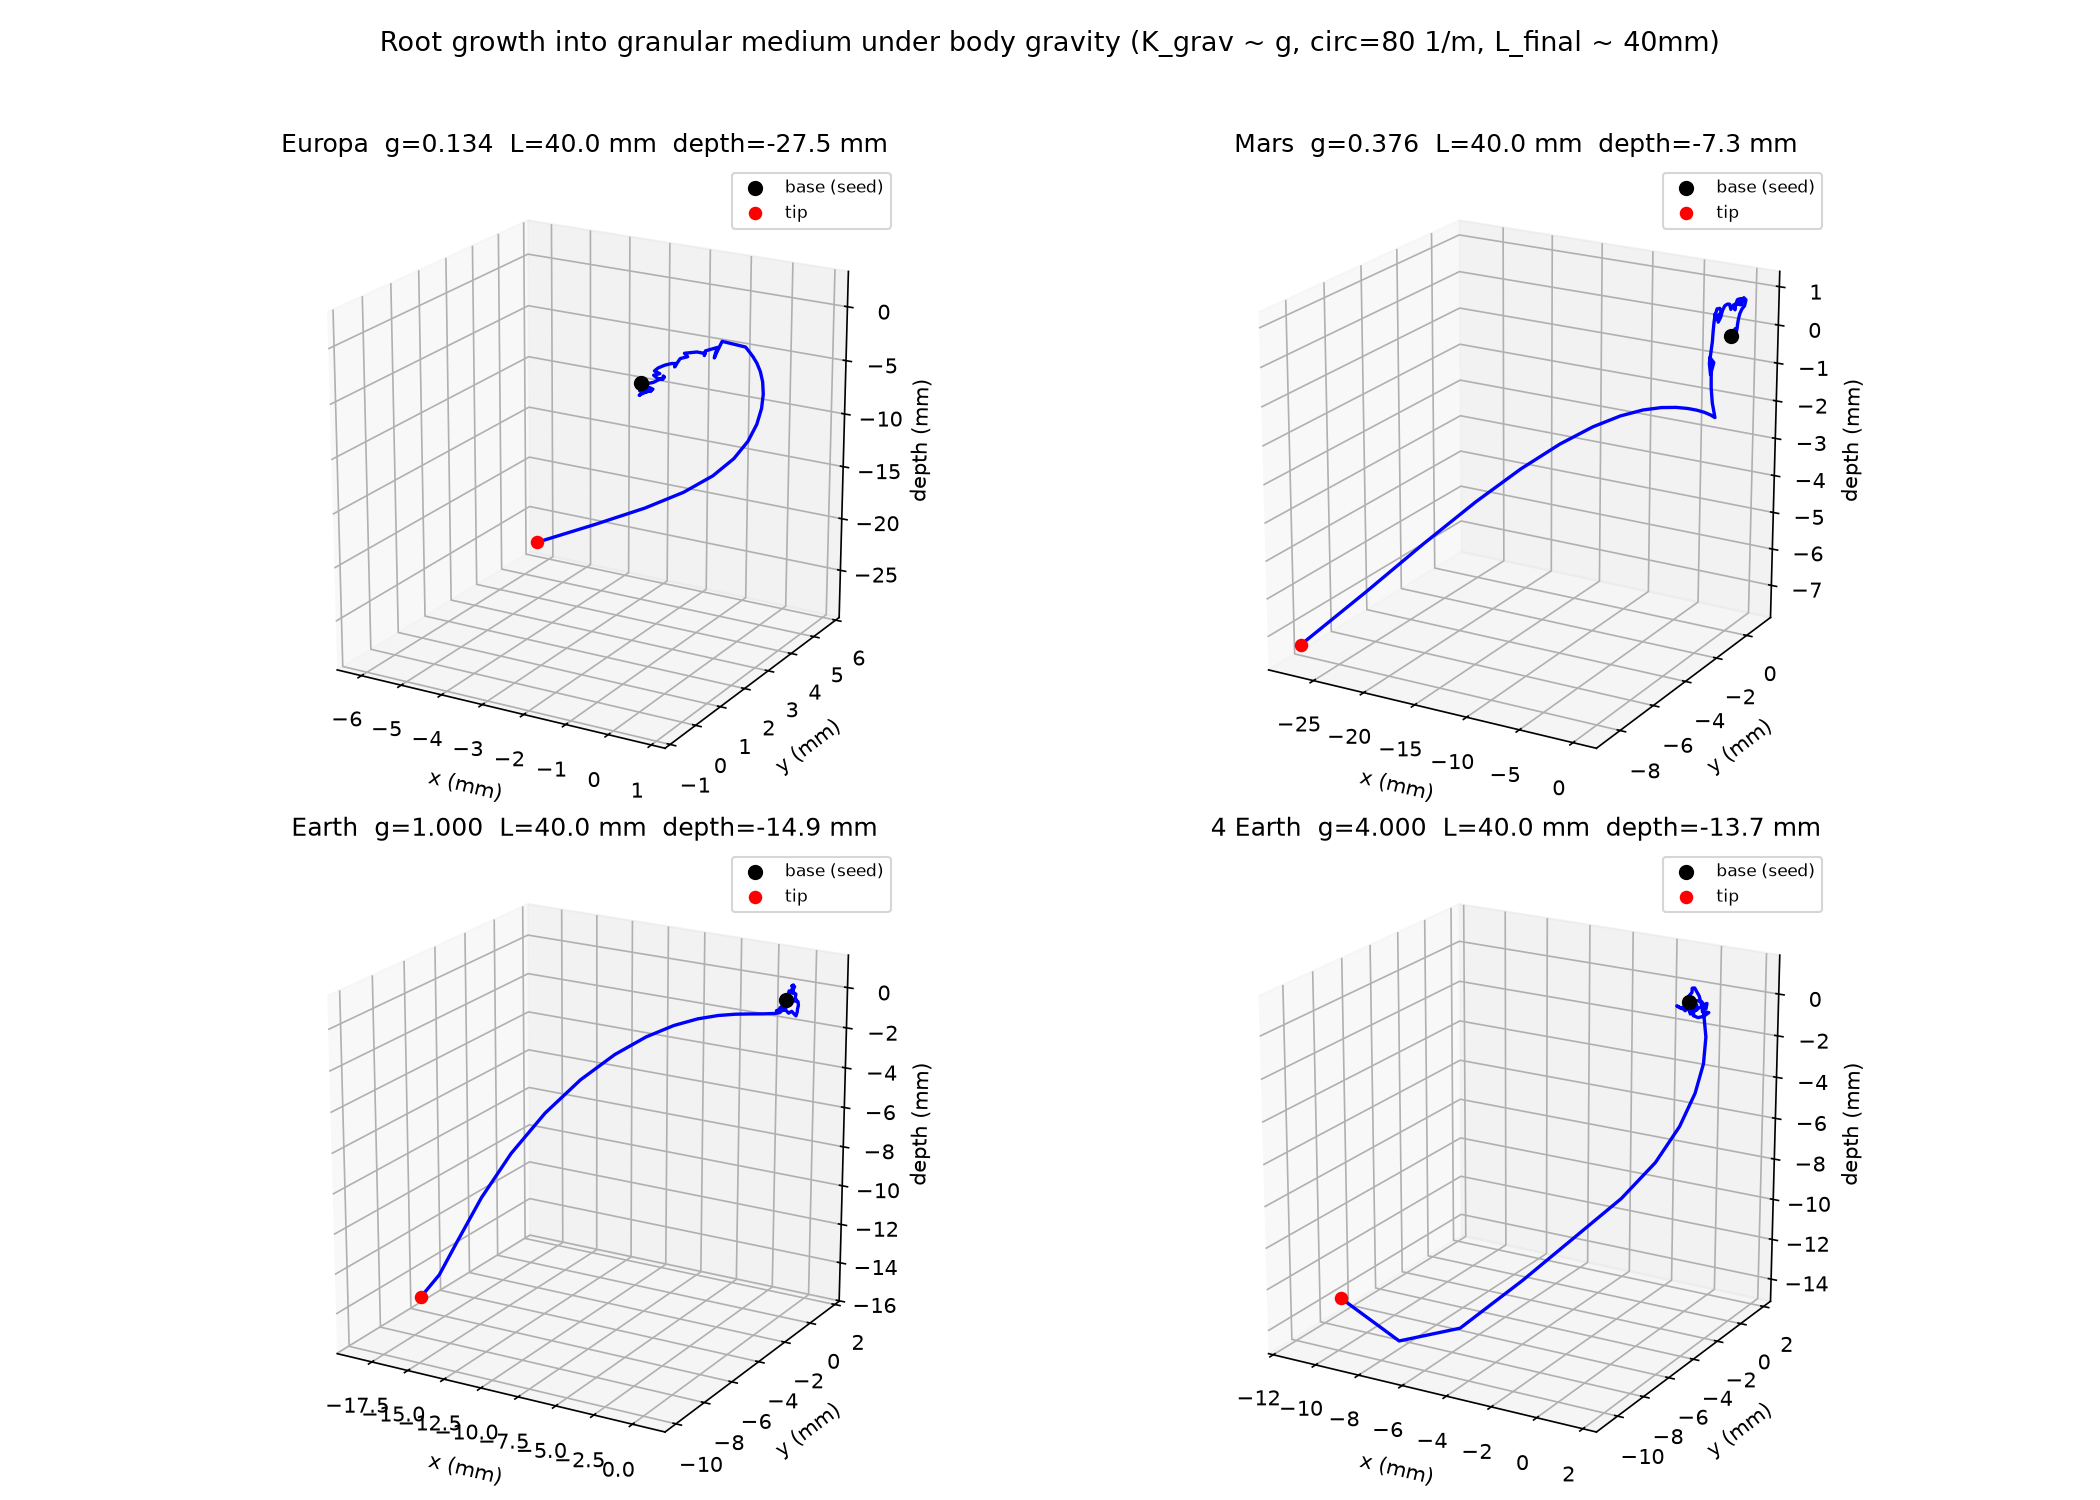
\includegraphics[width=0.8\textwidth]{figures/gravity_trajectories.png}
\caption{Three-dimensional tip trajectories for representative bodies of
Table~\ref{tab:gravity} (Europa, Mars, Earth, $4g_E$), rendered from the full
solved centreline. Burial decreases monotonically with gravity; at high $g$
the morphology is wandering and the tip is thrust-limited near the analytic
$z^{*}$.}
\label{fig:trajectories}
\end{figure}

\subsection{Morphology}
\label{sec:morph}

The morphology is wandering across the
whole gravity range (Fig.
\ref{fig:trajectories}), with two trends. As gravity increases, the
gravitropic gain \eqref{eq:grav} grows proportionally and the organ turns
more aggressively: the phase-averaged relative lateral excursion rises from
$\vartheta=0.081$ at Europa gravity to $\vartheta=0.170$
at $4g_E$ (the low-$g$ values sit within a narrow band of $0.07$--$0.12$). Because the mechanical moment that bends the tip scales as
$F_{\mathrm{tip}}L/B_1$, the achievable curvature saturates once
$F_{\mathrm{tip}}$ is capped by the medium or the thrust ceiling; large gains
therefore add tropic command faster than the mechanics can express it, and
all cases eventually saturate into the same wandering family. The vertical
efficiency is near zero in every case: it vanishes in the low-$g$ regime
because wandering dissipates the bulk of the elongation, and in the
high-$g$ regime because the thrust limit rotates the tip tangent toward the
horizontal (\eqref{eq:thrust}). Efficiency is thus a poor descriptor of these
growths; the realized depth, not a speed of descent, is the meaningful
quantity.

\section{Discussion}
\label{sec:discussion}

\subsection{Penetration as a controlled quantity under variable gravity}
The exact inverse law \eqref{eq:zstar} is the main quantitative output. It
states that, at fixed generative pressure $F_{\max}/A$ and fixed medium
constants, the quasi-static burial depth is inversely proportional to the
overburden, and nothing more. This is a statement about the medium (its
strength gradient is linear in $\rho g$) and about the organ (its generative
capability is finite and gravity-independent---a growing cell applies a
turgor pressure that does not change because the local gravity does). The
numerics confirm the law where it is testable (the $4g_E$ case sits at the
generative ceiling for a growing fraction of the run) and expose the
complementary regime where it is not yet operative, the length-limited and
wandering regime of low gravity. The
practical reading is direct. In a lunar or martian regolith the model
predicts that a 4 mm diameter root with a generative pressure of $F_{\max}/A
\simeq8$ kPa could in principle bury itself to $\sim$200 mm (Europa),
$\sim$160 mm (Moon) or $\sim$72 mm (Mars)
if its tropic controls kept it vertical; absent such control it wanders and
its realized burial is set by total length. At $4g_E$, by contrast, burial is
hard-capped near 7 mm; placing a seed or sensor at depth under supergravity
regimes requires either a much higher generative pressure (the ceiling
moves as $z^{*}\sim F_{\max}$ linearly) or a helper mechanism that improves
the medium (loosening, clod-forming agents).

\subsection{Relation to surface-morphology rod models}
The present model and the surface-pattern works \cite{sipos2022,porat2024}
share a mathematical backbone--a growing rod with intrinsic curvature--but
address different physical situations. In those works the organ grows on a
rigid, impenetrable plane and the pattern (straight, waving, coiling,
skewing) is selected by the interplay of gravitropism, growth and the
constraint of the plane; gravity appears as a fixed direction. Here the
medium is a yielding granular volume and the fundamental question is the
depth the organ can reach, not the pattern it draws on an interface; gravity
appears as a variable that rescales body force, medium strength and tropic
gain together. The two pictures are complementary rather than overlapping:
the interfacial studies validated the rod-mechanics machinery against
species-specific \emph{Arabidopsis} phenotypes, while the present analysis
targets a scaling law in a regime the interfacial studies do not cover. We
therefore cite those models as the closest related work, not as a template
followed here.

\subsection{Limitations and outlook}
The intentional simplifications are the following. (i) The regolith is an
isotropic Mohr--Coulomb material described by a lumped cone-bearing law
\eqref{eq:tipforce}; real soils are rate-, moisture- and
compaction-dependent, and the cone factors in \eqref{eq:conefactors} are the
classical quasi-static values. (ii) The rod is a single emergent organ with a
fixed cross-section and a fixed generative pressure; branching, taper,
grooves and hand-like tips are absent. (iii) The tropic gains and the growth
law are time-independent; there is no adaptation of circumnutation to
obstacles and no hydro-, chemo- or thigmotropism. (iv) The thrust ceiling is
enforced as a rigid angle constraint \eqref{eq:thrust} rather than as a soft
local slip law. (v) The stiffness is an optimistic upper bound, so $B_1$ is
larger than in living tissue; the morphology results are insensitive to this
because the achievable curvature saturates in any case. Parameters are
reported as indicative rather than matched to any species; the purpose is the
scaling, which is robust across the scanned ranges of stiffness, gain and
medium parameters. A natural extension is to let the root interact with a
lateral neighbour (introducing contact and friction between two growing
organs), which turns the same framework toward root intertwining and
clumping in dense sowing, and toward the collective rooting of small
regolith samples.

\section{Conclusion}
\label{sec:conclusion}

A growing root penetrates a granular medium by applying to it the generative
force of its tip against a bearing resistance that grows linearly with
overburden. We presented a minimal, numerically exact morphoelastic-rod
description of this process and showed that gravity enters it in three
separable places--self-weight, medium strength gradient and gravitropic
gain--with the consequence that burial obeys an exact $z^{*}\propto 1/g$ law
in the thrust-limited regime and switches to a length- and
wandering-limited regime at low gravity. The numerics verify the independence
of the control mechanisms and the law over a 30-fold range of gravitational
acceleration, and bound where a finite generative thrust stops a root from
making depth. The framework is cheap (minutes on a single core) and directly
reusable for forward estimates of root deployment on the Moon and Mars, for
compaction-avoidance in agricultural soils, and, with the addition of
organ--organ contact, for collective root behaviour.

\section*{Data availability}
The simulation code, the solver and the parameter tables used to produce
Tables~\ref{tab:control}--\ref{tab:gravity} and Fig.~\ref{fig:trajectories}
are publicly available at
\url{https://github.com/ogiannopoulou/root-burial-gravity}. All numerical
values reported are reproducible from the equations in the text,
the reference parameters of Table~\ref{tab:params}, and the scripts and
output data of that repository.

\bibliographystyle{unsrt}
\bibliography{references}

\end{document}